\section{Results}
\label{results}

Borrowing again from Flaxman 2014, the models were evaluated on a variant of $R^2$ that captures the reduction in variance from each model component. The error from predicting solely on the spatial expectation $e_s$ serves as a baseline for comparison:

$$ 1 - \frac{\sigma_{s,t}(n_{s,t}- \hat{n_{s,t}})^2}{\sigma_{s,t}(n_{s,t} - e_{s})^2}$$


\subsection{Long Term Predictions}

 Weekly traffic collision and injury data was aggregated to the level of New York City neighborhoods for this set of experiments. While data is available for the past five years, there appears to have been a reporting error for part of 2016 which made the year of data problematic for both model fitting and testing. It would have been ideal to fit the model based on multiple years of data leading up to the latest available data, but given the unreliable data the best alternative was fitting the LGCP on three years of data from July 2012 to July 2015, and leaving the following 52 weeks for out-of-sample prediction.  \par


 \begin{figure}[h!]
   \caption{A Gaussian Process fit to weekly pedestrian injuries in New York City from 2012 to 2015. The dotted line shows where out of sample prediction begins.}
   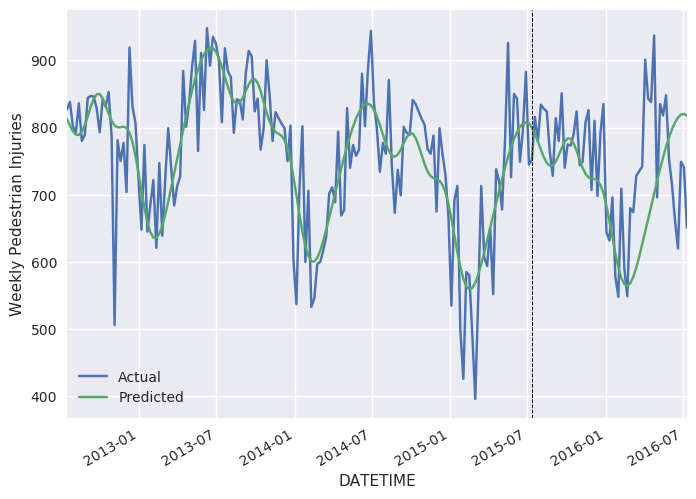
\includegraphics[width=0.5\textwidth]{citywide_predictions}
 \end{figure}

\todo{discussion of confidence?}

Since the kernel components are all additive they can provide an interpretable decomposition of the model components. There is clear annual periodicity in the model, which is also confirmed by the period parameter fitted being almost exactly 52. The linear kernel component also suggests a small downward long-term trend in pedestrian injuries.

\todo{table of parameters}


\begin{figure}[h!]
  \caption{}
  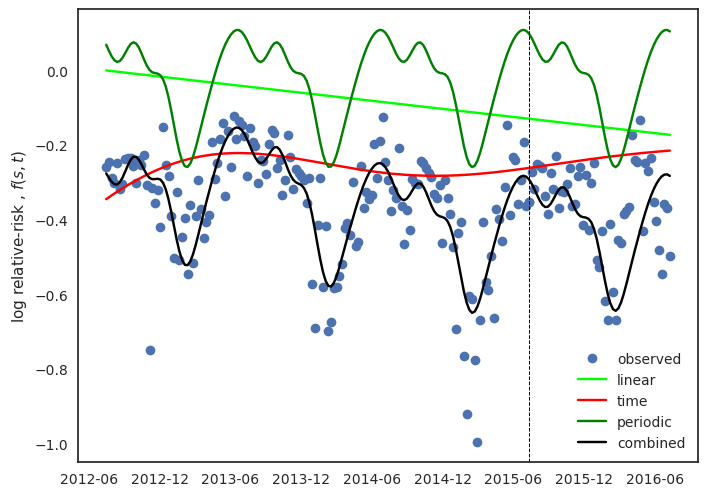
\includegraphics[width=0.5\textwidth]{citywide_var_decomp}
\end{figure}

 \todo{chart of data errors}


 \subsection{Neighborhood Predictions}

 Neighborhood level predictions of pedestrians injuries were added
 New York City defines official Neighborhood Tabulation Areas (NTAs), which were used as the geographic areas of interest. The model was fit on the 29 official NTAs in the borough of Manhattan using 52 weeks of weekly pedestrian injury data. The spatial component was calculated from the distance between centroids for each NTA. \par

 \begin{figure}[h!]
   \caption{Manhattan's 29 neighborhoods, with red dots indicating the centroid used for calculating distance.}
   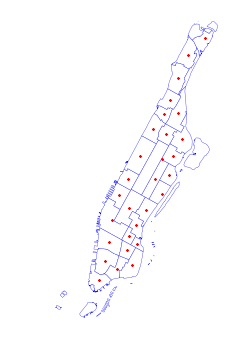
\includegraphics[width=0.5\textwidth]{mn_centroids}
 \end{figure}

 \begin{figure}[h!]
   \caption{Relative risk scores for Manhattan neighborhoods. Midtown is roughly twice as dangerous for pedestrians than Manhattan as a whole.}
   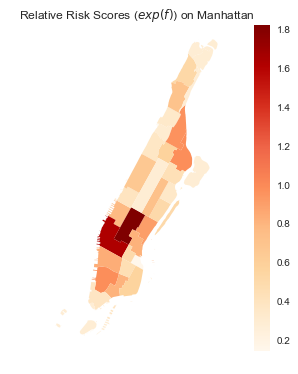
\includegraphics[width=0.5\textwidth]{mn_f_score_map}
 \end{figure}



 \todo{data example}
 \todo{NTA map}


\subsection{Short Term Forecasting}
